\documentclass{article}
\usepackage[utf8]{inputenc}
\usepackage{graphicx}
\usepackage{subcaption}
\bibliographystyle{plain}

%\title{libbdsg and libhandlegraph: High-performance sequence graph implementations for graphical pangenomics}
\title{Succinct dynamic sequence graphs} % for graphical pangenomics}
  %libbdsg and libhandlegraph: High-performance sequence graph implementations for graphical pangenomics}
\author{Jordan M. Eizenga \and Adam M. Novak \and Emily Kobayashi \and Cecilia Cisar \and Benedict Paten \and Erik Garrison}

\newcommand{\vocab}{\textbf}

\begin{document}

\maketitle

\begin{abstract}

Pangenomics is a growing field within computational genomics.
Many pangenomic analyses use bidirected sequence graphs as their core data model.
However, implementing and correctly using this data model can be difficult, and the scale of pangenomic data sets can be challenging to work with.
Here we present two C++ libraries with Python bindings, \texttt{libbdsg} and \texttt{libhandlegraph}, which share a simple, field-proven interface designed to expose elemental features of these graphs while preventing common graph manipulation mistakes.
Through experiments with a diverse collection of pangenome graphs, we demonstrate that these tools allow for efficient construction and manipulation of large genome graphs with dense variation.

\end{abstract}

\section{Introduction}

With falling sequencing costs, the genomics community has sequenced increasingly many individuals within certain species.
For example, hundreds of thousands of deeply sequenced human genomes are now available.
The novel challenges of analyzing data sets of this scale have led to the development of \vocab{computational pangenomics}, which focuses on the analysis of populations of genomes rather than individuals \cite{computational2016computational}.

Much of the research in computational pangenomics has coalesced around graph-based approaches for representing populations of genomes \cite{Paten_2017}.
Unlike conventional string-based representations, graph data structures provide a coherent modeling language to represent different types of genomic variation like substitutions, insertions, deletions, and more complex genomic events.
They support the compact representation of many-way relationships, such as whole genome alignments, between related genomes \cite{kehr2014genome}.

Graph-based data structures also present new computational challenges.
In addition to sequence, graphs must represent topology.
Given the size of many genomes of interest, this can be quite demanding on computer memory.
Further, there is significant impetus to make the graph data structures computationally efficient, since they are frequently the core data structure in pangenomics applications.

Genome graphs that include small variants from a large population of eukaryotic genomes can contain hundreds of millions of nodes and edges.
While the total information content in such models is only incrementally more than that require to represent the total sequence set of the pangenome, using naive data structures to identify and provide random access to elements of these graphs has very high memory costs.

The variation graph toolkit (\textsc{vg}) \cite{Garrison_2018} provides a cautionary tale of such an implementation.
It uses full width machine words as identifiers for elements, and stores the graph and its topology in a set of hash tables linking these identifiers to raw pointers.
Loading the 1000 Genomes Project's variant set into the \textsc{vg} toolkit can require $\approx$30 times as much memory as the serialized representation, consuming more than 300 GB of memory \cite{Garrison_2019}.

Although \textsc{vg} provides a memory-efficient succinct representation of the graph (\textsc{xg}) that is used during read mapping and variant calling, it is static and does not allow for dynamic updates to the graph.
In result, graph modifying steps in pangenomic analysis pipelines must be applied to large graphs by breaking the graph into smaller pieces.
This is unfortunately not tenable for all graphs.
For instance, many whole genome alignment and assembly graphs consist of a single giant component that cannot be partitioned easily.

To overcome this limitation, we have developed three new graph genome data structures that are both succinct, in requiring working memory in the order of the information content of the graph, \emph{and} dynamic, in that they allow efficient updates and edits to the graph.
Here, we compare the performance of these data structures to those in \textsc{vg} and \textsc{xg} on a diverse collection of genome graphs obtained during our work in graphical pangenomics.

In addition to demonstrating the possibility of working with large, complex graphs in small amounts of memory, these implementations expose a common API based on the \textsc{HandleGraph} model.
This model provides a consistent, reliable interface to genome graphs based on their fundamental units.

%To support reuse by other researchers,
We package these implementations behind equivalent C++ and Python APIs in \texttt{libbdsg}.
This software library will reduce the need for individual research groups to continually reimplement these core data structures.
These dynamic \textsc{HandleGraph} libraries will ease the development of algorithms that work on large, complex pangenome graphs by making it easy to store them in reasonable amounts of working memory and manipulate them in reasonable amounts of time.

%In response, we present a suite of

%We have developed a stack of C++ libraries providing high-performance sequence graphs for graphical pangenomics applications.
%We also provide Python bindings so the components are accessible to Python developers as well.

%The C++ stack consists of two components.
%First, we have developed an abstract interface for sequence graphs, based on our experience in the VG project.
%Second, we have developed three concrete implementations of the sequence graph interface, which make different trade-offs between speed, memory, and complexity, and which attempt to provide good coverage of the design space. 

\section{Implementation}

\subsection{Data model}

Our libraries adopt node-labeled bidirected graphs as a formalism for sequence graphs.
In a bidirected graph, nodes are considered to have left and right ``sides'', and edges connect two sides rather than two nodes.
In bidirected sequence graphs, a node's sides correspond to the 5' and 3' ends of its DNA sequence. 

Paths through a bidirected graph must leave a node out of the opposite side that they enter it.
We interpret paths that traverse a node from the 3' side to the 5' as using the node's reverse complement strand, which provides a natural means to encode DNA strandedness.
Specific paths correspond to sequences of interest, such as reference genomes or annotations (subsequences) of them.
Because paths like these are so frequently important in practice, our formalism also includes paths as a first class object, embedded in the graph.

\subsection{The handle graph interface}

The \texttt{libhandlegraph} library describes a generic interface that exposes basic operations on our sequence graph data model.
The interface uses ``handles'', which are opaque numeric references modeled after the concept of a file handle, in order to remain agnostic about the backing implementation of the graph.

The \textsc{HandleGraph} model focuses on five fundamental entities in the bidirected sequence graph:

-- \emph{Handles} identify one strand of a DNA sequence in the graph.

-- \emph{Nodes} identify pairs of complementary DNA strands, and have unique numerical identifiers (IDs).

-- \emph{Edges} link pairs of handles.

-- \emph{Paths} represent sequences as walks through the graph, and are composed of \emph{steps} that describe a path's traversal of a particular handle.


The \texttt{libhandlegraph} interface requires sequence graph implementations to be able to provide or consume these handles for basic queries.
%The handles are then passed back to the API to refer to these entities when performing operations and making queries.
For instance, we might obtain a handle from an implementation by querying a node's ID and providing an orientation, while another function provided in the implementation would map the handle back to a given node ID.
We can obtain reference to a path by its name (e.g. ``chr22''), and then iterate over the series of step handles in the path to follow its course through the graph.
Starting from a given handle, we can follow its outgoing edges along the same strand and direction to explore the topology of the graph.

The actual contents of a handle are unspecified, which gives significant flexibility to the implementation.
An implementation need not actually store the handle in its unpacked form.
Handles might be implicitly represented internally, in minimal space.

One benefit of this design is that any algorithm designed for one handle graph implementation can be applied to all other implementations.
Another is that, since the user works only through handles, their ability to make mistakes can be restricted.
For example, the interface can enforce the constraints on paths through bidirected graphs during edge traversal.
In general, the interface can be made memory safe for external users by eliminating reference to raw pointers or other direct access to graph elements.

%This prevents common mistakes that the developers identified in their work on the VG project.
%Taken together, these benefits enable code that focuses on the algorithms rather than on boilerplate bookkeeping.

\subsection{Graph implementations}

The \texttt{libbdsg} library consists of four concrete implementations of the handle graph interface.
Each implementation represents a different tradeoff in terms of speed, memory use, and capabilities.
All of the implementations except XG are dynamic.

\subsubsection{HashGraph}

This implementation has speed as its primary goal.
The core adjacency list is implemented using a high performance hash table.
Most of the smaller component data structures are uncompressed STL objects, so they can easily be computed on in the native in-memory format.
Embedded paths are implemented as doubly-linked lists.
This implementation is most appropriate for small graphs (from small genomes or small regions of larger genomes) or for high-memory compute environments.

\subsubsection{PackedGraph}

This implementation focuses on having a low memory footprint.
Most of its component data structures are---conceptually speaking---linked lists.
However, they are implemented using vectors of bit-compressed integers, where pointers are produced by treating some of the integer entries as indexes into the vector that contains them.
The bit-width can be chosen dynamically without affecting the amortized asymptotic run time of graph operations in the typical case that the $i$-th entry in the vector is $O(i)$.
The vector uses a windowed bit compression scheme in which only one value within a window is maintained at its full bit-width.
The remaining entries are represented as differences from this value.
In the typical case where adjacent entries in the vector are highly correlated, this helps keep the bit-width low and thereby the compression high. 

\subsubsection{ODGI}

\textsc{odgi} is based on a node-centric encoding of the graph that is designed to improve cache coherency when traversing or modifying the graph.
This encoding is split between graph topology and paths, which was found to be important to yielding a good balance of runtime performance and memory usage on real-world graphs with large path sets.
Each node's its sequence and inbound and outbound edges are encoded in a byte array using a variable-length integer encoding scheme.
Edges are described in terms of a relative offset between the rank of this node in the sorted array of nodes of the graph and the node to which the edge arrives (or from which it emanates).
The set of steps traversing each node is recorded in a second dynamic integer vector of fixed width entries, compressed so that only largest integer entry is stored at full width \cite{prezza2017framework}.
Each step links a path identifier, relative ranks of the previous and successive node traversals on the path, and the rank of the next or previous step among the path steps recorded at that node.
This path encoding scheme is similar to that used in the dynamic GBWT \cite{Siren_2019}, but differs in that the paths are not prefix-sorted but are added in an arbitrary order.
%It is designed to exploit the sparse and orderable nature of genome graphs.
Provided each path step tends to move only a short distance in the sorted nodes of the graph (e.g. from $n_{5} \to n_{7}$), then the maximum bitwidth of the path vector will be low, resulting in good compression.

%Longer-range jumps do occur, but they tend to be more rare.
%Modifying path step records can be expensive, but when the number of traversing paths is relatively small, it remains in higher caches and can be accomplished efficiently.

\subsubsection{XG}

Unlike the others, this implementation is static.
This permits a more powerful set of efficient queries from the graph, especially from paths.
The encoding is designed to balance speed and low-memory usage.
The topology of the graph is encoded in a single vector of bit-compressed integers, which promotes cache-efficiency.
Rank and select operations on compressed bit-vectors are used to provide random access over the variable-width records.
Embedded paths are encoded in variable-length integer vectors with Elias gamma encoding.
Rank and select operations from bit vectors also provide queries by base-pair position along paths.

\section{Evaluation}

\subsection{Human genome with structural variants}

We measured the performance during core operations of the four graph implementations and the graph class from the popular VG software.
In particular, we measured 1) memory usage while constructing a graph, 2) time to construct a graph, 3) memory usage when loading an already-constructed graph, and 4) time to access nodes, edges, and steps of a path.
The presented results are from a graph constructed from the structural variants of the HGSVC.
The comparison generally follows our expectations based on the design principles behind each implementation (Figure \ref{fig:hgsvc}).

\subsection{Genome graph collection}

To evaluate the relative change in performance of the methods over a wide variety of different graphs, we applied each to 2299 graphs collected during our research on graphical pangenomics.
For each graph and graph implementation, we measured construction and load time and memory, query time, and various graph properties including size, edge count, cyclicity, and path depth.
We summarize these results in Figure \ref{fig:prof}.

For graph construction and loading, we observe similar trends as for the HGSVC graph.
\textsc{vg}'s performance in terms of memory usage is very poor, both during construction and load.
For construction and load, all models exhibit largely linear scaling characteristics, outside of very small graphs where static memory overheads dominate.
\textsc{PackedGraph} yields the best memory performance for larger graphs (which are mostly the chromosomes of the 1000 Genomes Project graph), while for the medium-sized graphs in the collection (of ~1 Mbp), \textsc{odgi} requires less memory better.

For graph queries and enumeration, the relative performance of the models is largely maintained across the entire range of graph sizes.
However, we observe that the hash-based models (\textsc{vg} and \textsc{HashGraph}) have very good performance for smaller graphs (in handle and edge enumeration) but decrease in throughput as the graph size increases.
Smaller, less significant decreases in performance can be seen for the other implementations.
For path enumeration, the highest-performing methods are \textsc{xg} and \textsc{HashGraph}, which store paths in linear arrays, are approximately 10 times faster than \textsc{odgi}, whose relativistic path storage is apparently costly to traverse.

% \section{Discussion}

% The \texttt{libhandlegraph} and \texttt{libbdsg} C++ libraries provide high-performance sequence graph implementations that encourage quality coding. Python bindings are also available. This software can help developers write future pangenomics applications. 

% TODO: we should write a guide on GitHub for how to use

\bibliography{references.bib}

\begin{figure}
	\begin{center}
		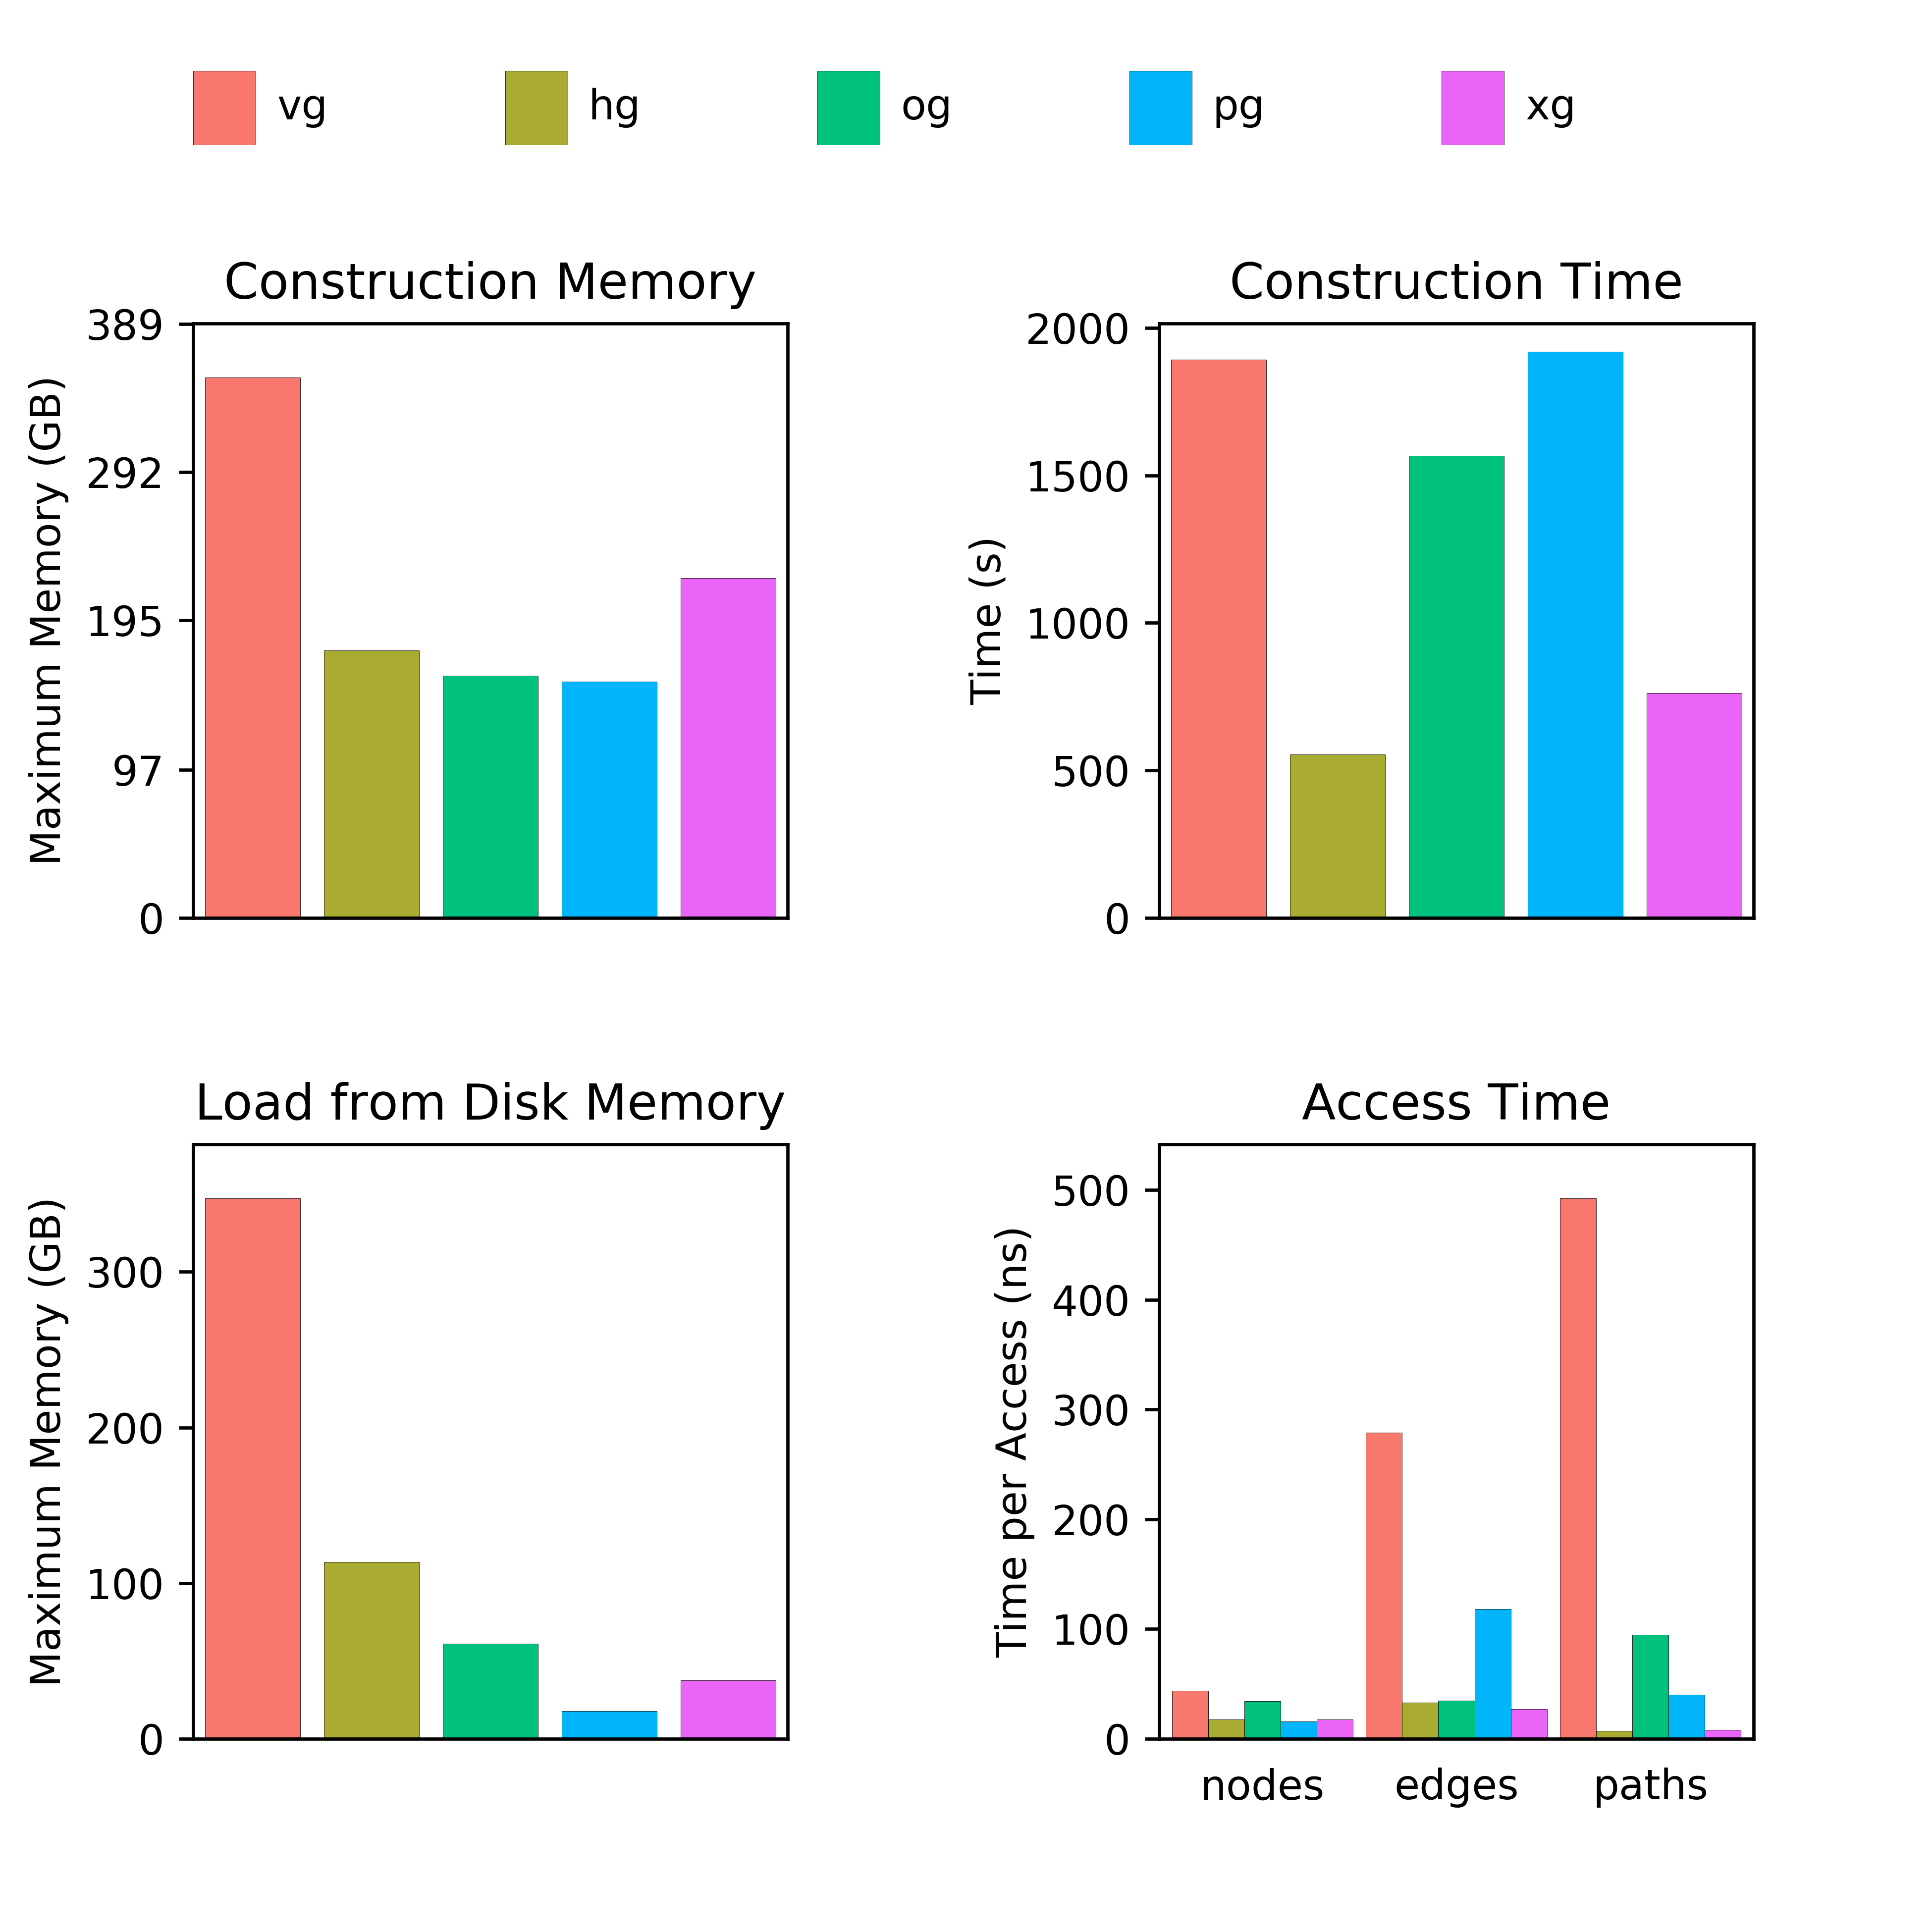
\includegraphics[width=.75\textwidth]{figures/HGSVC_sorted_gfa.png}
	\end{center}
	\caption{{\label{fig:hgsvc} \textbf{Performance on a graph of structural variants from the HGSVC.} All four new graph implementations compare favorably to VG. PackedGraph tends to be the most memory efficient, HashGraph tends to be the fastest, and ODGI is balanced in between. XG provides good performance on both memory usage and speed, but it is static.}}
\end{figure}

\begin{figure}
  \begin{subfigure}[t]{0.5\textwidth}
    \centering
    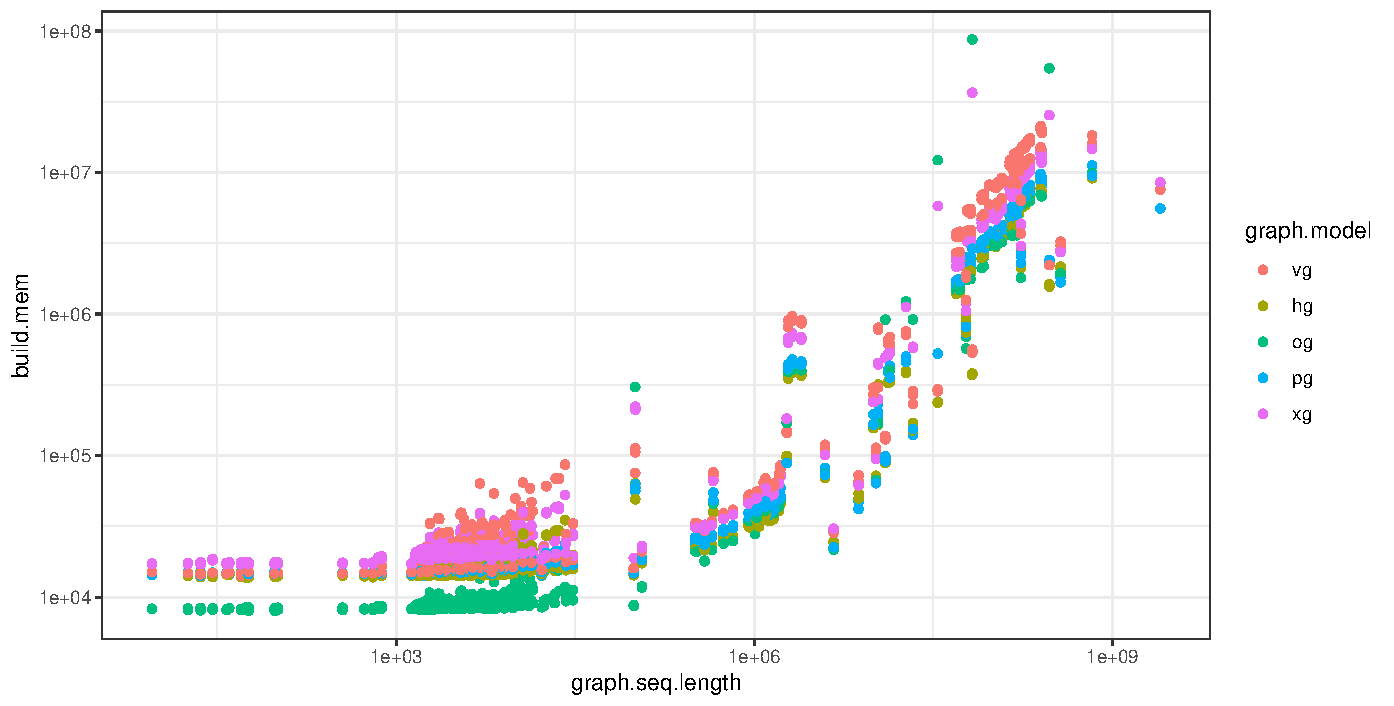
\includegraphics[width=1.0\textwidth]{figures/build_mem.pdf}
    \caption{build memory}
  \end{subfigure}
  \begin{subfigure}[t]{0.5\textwidth}
    \centering
    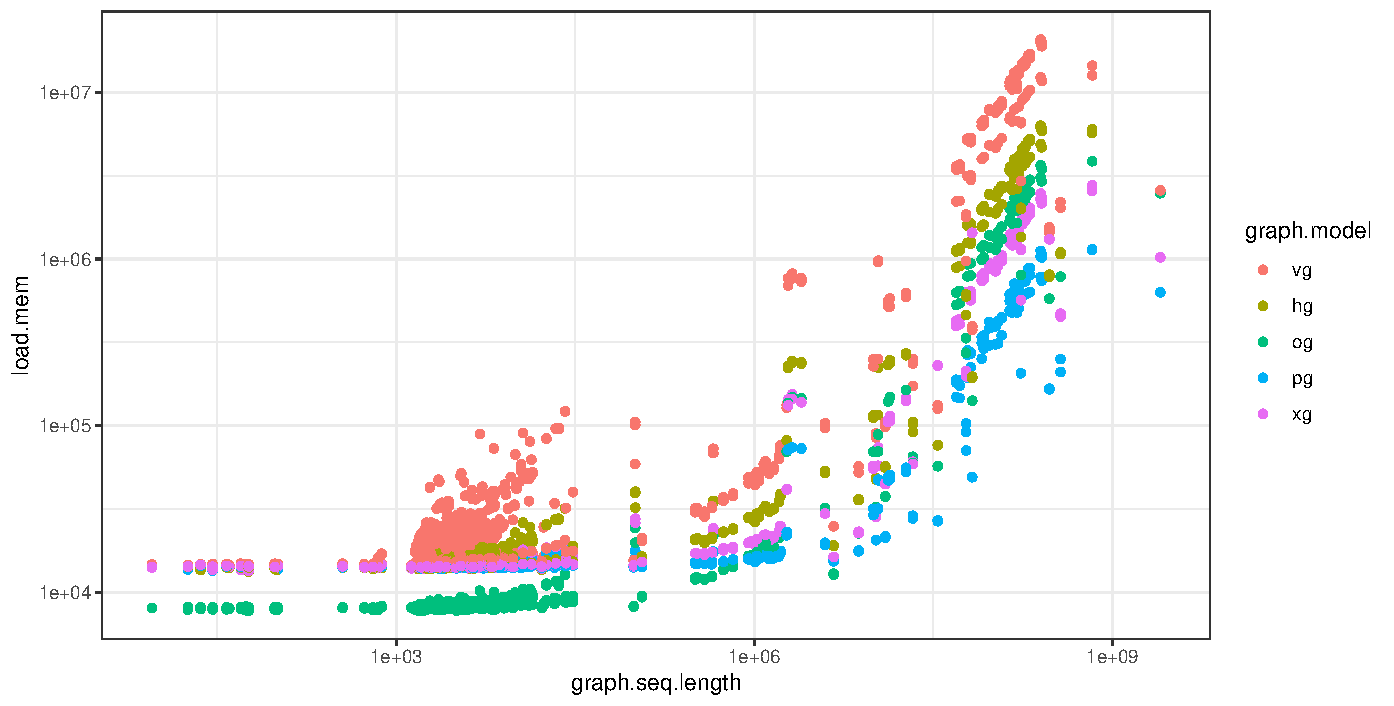
\includegraphics[width=1.0\textwidth]{figures/load_mem.pdf}
    \caption{load memory}
  \end{subfigure}
  \begin{subfigure}[t]{0.5\textwidth}
    \centering
    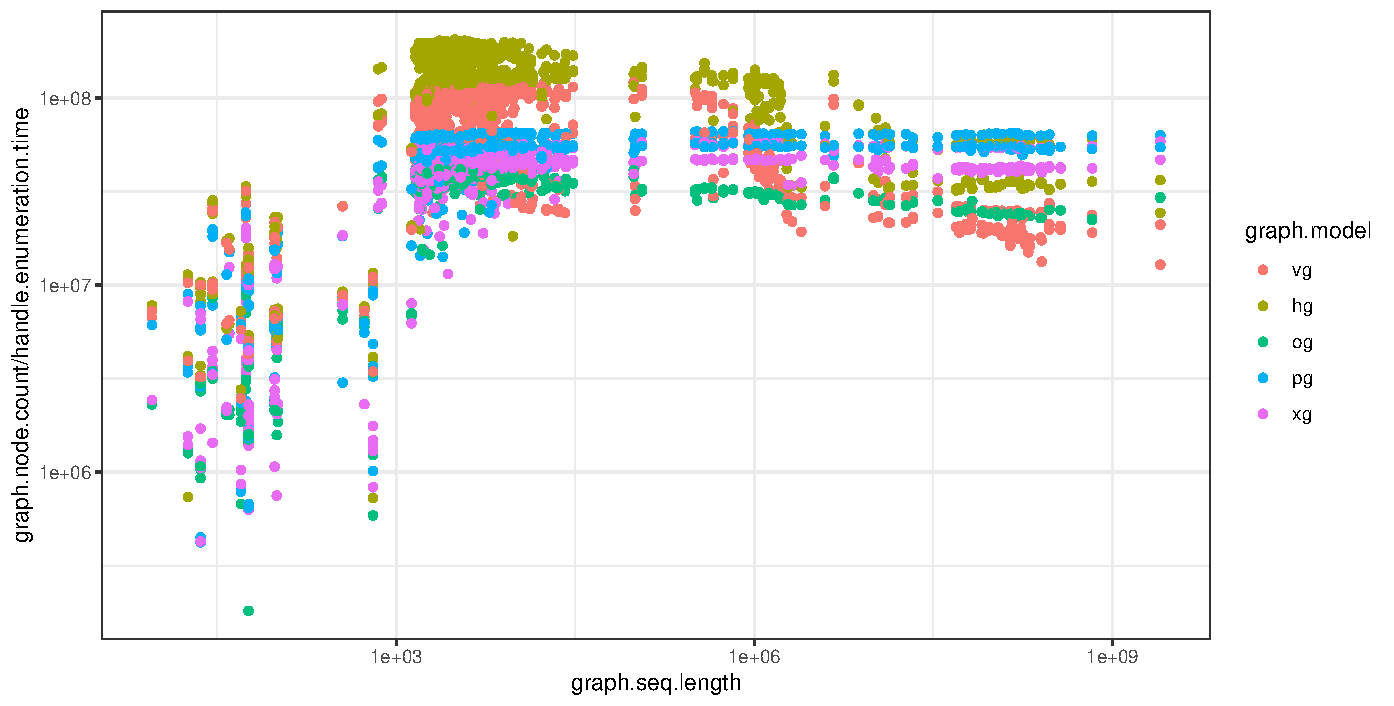
\includegraphics[width=1.0\textwidth]{figures/handle_enumeration_time.pdf}
    \caption{handles/second}
  \end{subfigure}
  \begin{subfigure}[t]{0.5\textwidth}
    \centering
    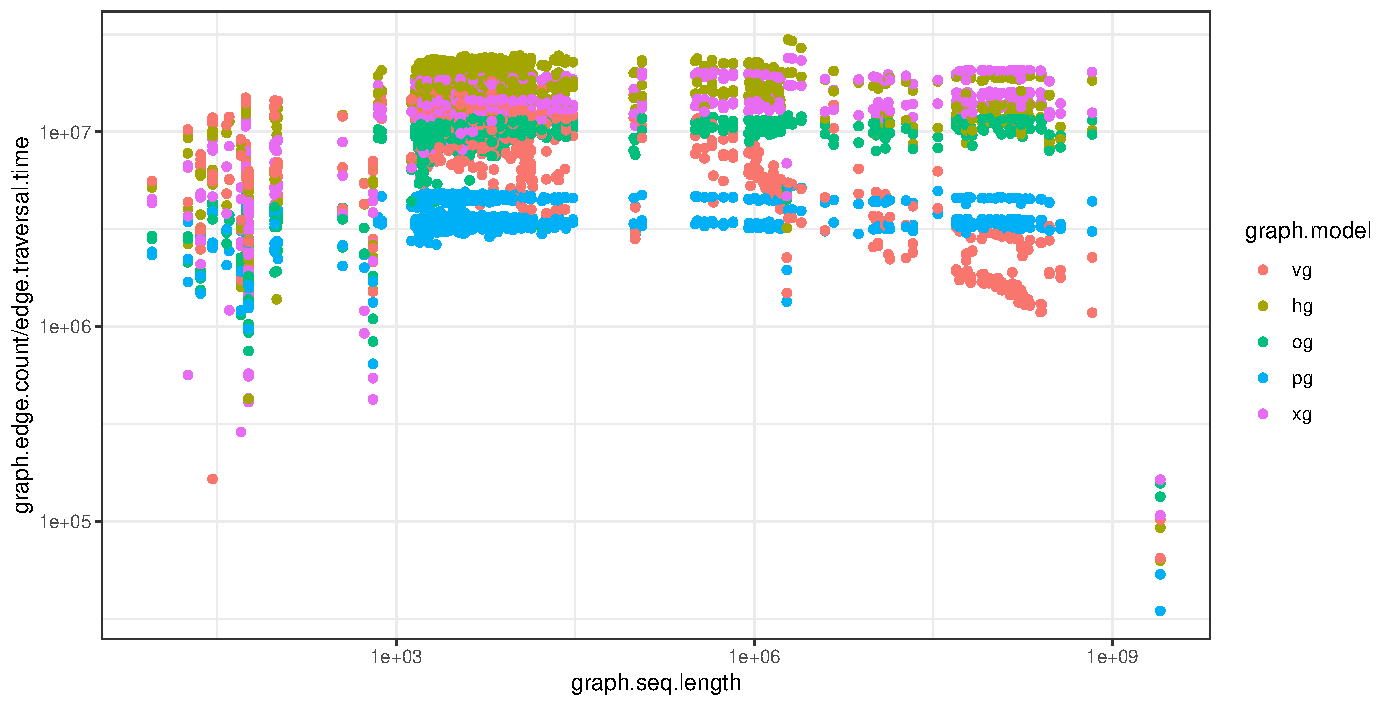
\includegraphics[width=1.0\textwidth]{figures/edge_enumeration_time.pdf}
    \caption{edges/second}
  \end{subfigure}
  \begin{subfigure}[t]{0.5\textwidth}
    \centering
    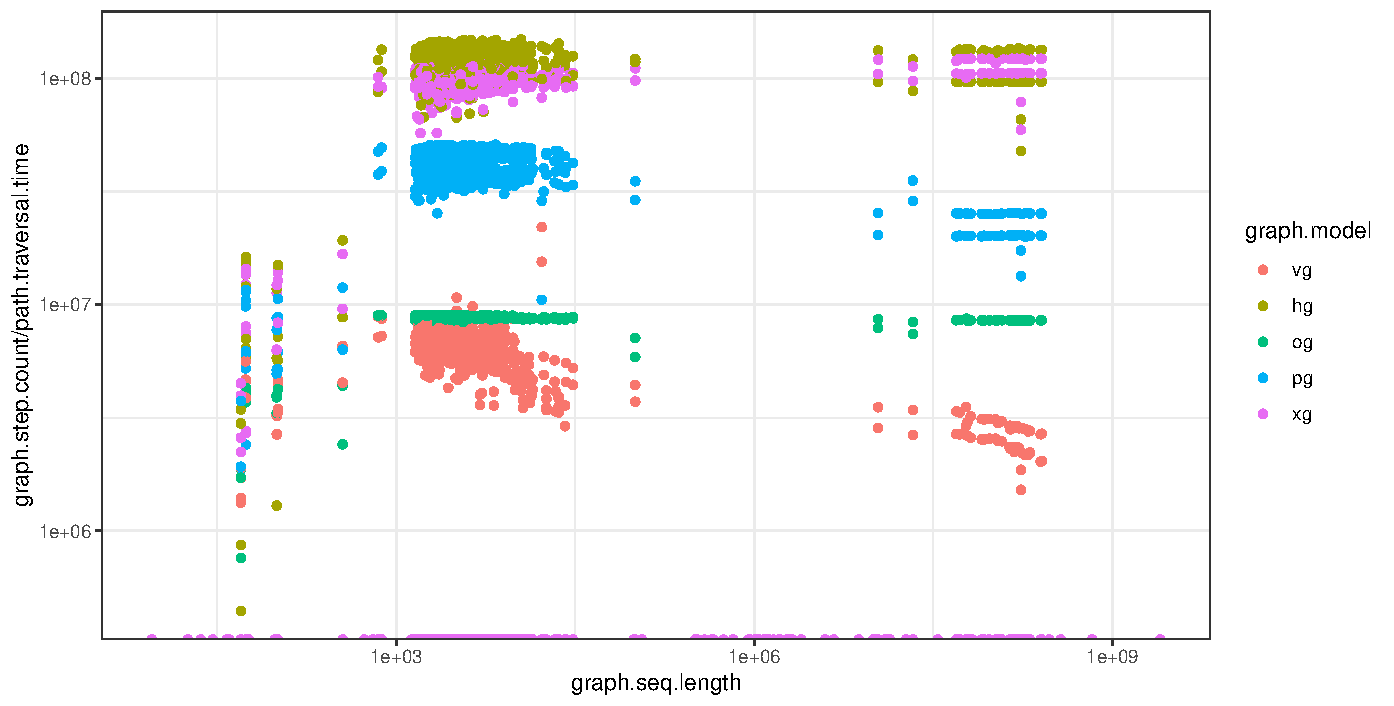
\includegraphics[width=1.0\textwidth]{figures/step_enumeration_time.pdf}
    \caption{path steps/second}
  \end{subfigure}
  \begin{subfigure}[t]{0.5\textwidth}
    \centering
    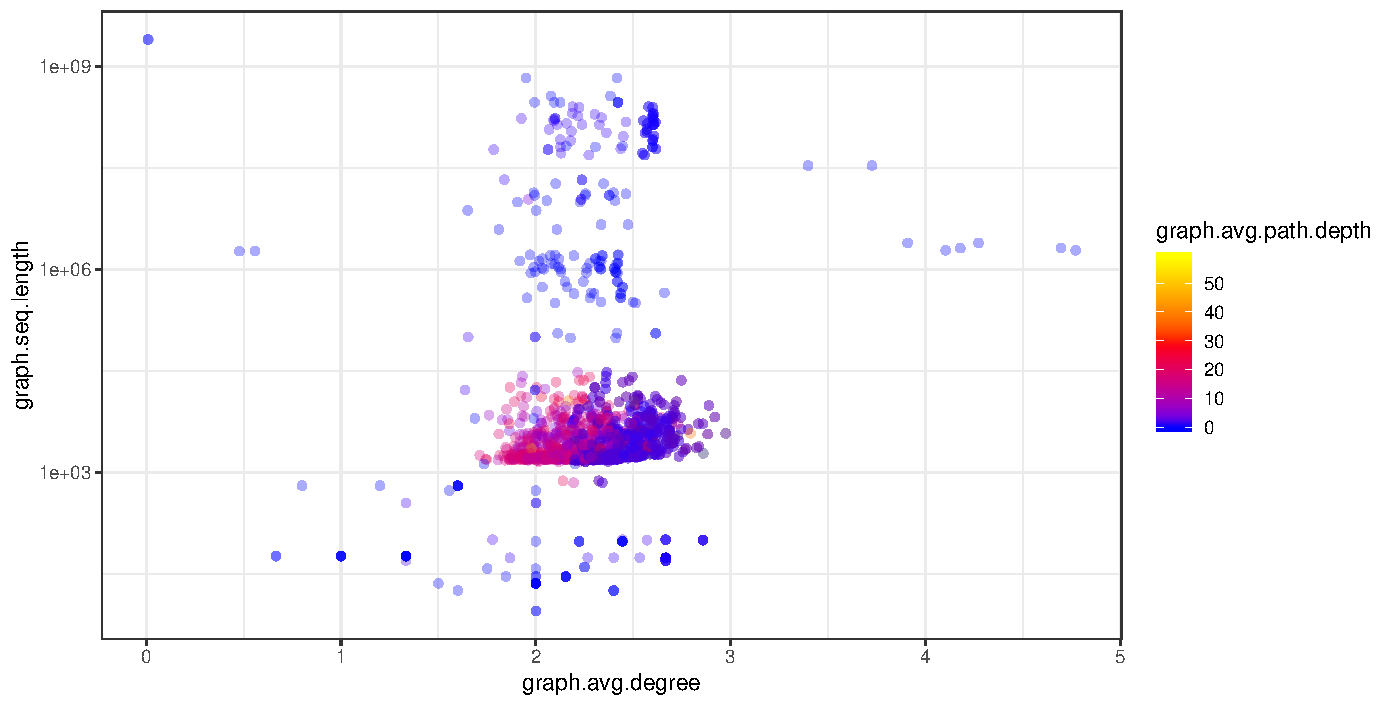
\includegraphics[width=1.0\textwidth]{figures/graph_summary.pdf}
    \caption{graph properties}
  \end{subfigure}
  \caption{
    \label{fig:prof}
    \textbf{Performance of models on the graph collection.}
    }
\end{figure}



\end{document}
